\documentclass[12pt, twoside]{article}
%\documentclass[12pt, twoside]{article}
\usepackage[letterpaper, margin=1in, headsep=0.2in]{geometry}
\setlength{\headheight}{0.6in}
%\usepackage[english]{babel}
\usepackage[utf8]{inputenc}
\usepackage{microtype}
\usepackage{amsmath}
\usepackage{amssymb}
%\usepackage{amsfonts}
\usepackage[nomessages]{fp} %\FPeval{\var-name}{2*sin(pi/6)}
\usepackage{siunitx} %units in math. eg 20\milli\meter
\usepackage{yhmath} % for arcs, overparenth command
\usepackage{tikz} %graphics
\usetikzlibrary{quotes, angles, arrows, arrows.meta}
\usepackage{pgfplots}
\usepgfplotslibrary{fillbetween}
\pgfplotsset{compat=1.16}
\usepackage{graphicx} %consider setting \graphicspath{{images/}}
\usepackage{parskip} %no paragraph indent
\usepackage{enumitem}
\usepackage{multicol}
\usepackage{venndiagram}

\usepackage{fancyhdr}
\pagestyle{fancy}
\fancyhf{}
\renewcommand{\headrulewidth}{0pt} % disable the underline of the header
\raggedbottom
\hfuzz=2mm %suppresses overfull box warnings

\usepackage{hyperref}

\fancyhead[LE]{\thepage}
\fancyhead[RO]{Markscheme}
\fancyhead[LO]{La Scuola d'Italia / Dr.\ Huson / IB Math 12 \\* 3 November 2026}

\begin{document}
\subsubsection*{3.2 Classwork: Transformations of Trigonometric Functions --- Markscheme}

\begin{enumerate}[itemsep=0.3cm]

%--- Problem 1: f(x) = 4sin(2(x - pi/6)) - 1: describe the transformations from y = sin x; amplitude, period, range; sketch with exact max and min [10 marks] ---
\item[1.] [Maximum mark: 10]

$f(x) = 4\sin\!\left(2\left(x - \frac{\pi}{6}\right)\right) - 1$

\textbf{(a)} Vertical stretch, scale factor $4$ \hfill \textbf{A1}

Horizontal stretch, scale factor $\frac{1}{2}$ \hfill \textbf{A1}

Horizontal translation $\frac{\pi}{6}$ to the right \hfill \textbf{A1}

Vertical translation $1$ down \hfill \textbf{A1}

\emph{``Describe fully'' needs words (markscheme-spec \S19). One mark per
transformation, each with its type, direction and size. Accept
``horizontal compression by a factor of 2'' for the horizontal stretch.
The vertical translation must say ``down''. Accept
``translation by $\binom{\pi/6}{-1}$'' for both translation marks.
Reject ``move''. A correct chain of equations with no words earns at most
1 mark.}

\emph{Order: the horizontal stretch must come before the translation of
$\frac{\pi}{6}$ right, and the vertical stretch before the translation
down. Also fully correct: translate $\frac{\pi}{3}$ right, then stretch
horizontally with factor $\frac{1}{2}$. Deduct 1 mark for a wrong order.
Wrong methods, each A0 for that transformation: translation
$\frac{\pi}{6}$ left; horizontal stretch with factor $2$.}

\textbf{(b)} amplitude $= 4$ \hfill \textbf{A1}

period $= \dfrac{2\pi}{2} = \pi$ \hfill \textbf{A1}

range: $-5 \le y \le 3$ \hfill \textbf{A1}

\emph{Accept $[-5,\ 3]$ or $-5 \le f(x) \le 3$. Strict inequalities earn
A0. Wrong methods: period $4\pi$ ($2\pi \times 2$) earns A0; range
$-4 \le y \le 4$ (vertical translation ignored) earns A0.}

\begin{minipage}[t]{0.5\textwidth}
\textbf{(c)} Sine-wave shape on $0 \le x \le \pi$, starting and ending at
$y \approx -4.46$, one maximum and one minimum \hfill \textbf{A1}

Maximum $\left(\dfrac{5\pi}{12},\ 3\right)$ \hfill \textbf{A1}

Minimum $\left(\dfrac{11\pi}{12},\ -5\right)$ \hfill \textbf{A1}
\end{minipage}
\hfill
\begin{minipage}[t]{0.44\textwidth}
\vspace{0pt}
\begin{tikzpicture}[xscale=0.44, yscale=0.4]
  \draw[thin, color=gray!50] (0,-5) grid (12,4);
  \draw[->] (0,0) -- (12.6,0) node[right] {$x$};
  \draw[->] (0,-5.3) -- (0,4.5) node[above] {$y$};
  \foreach \v in {-5,3} \node[left, font=\scriptsize] at (0,\v) {$\v$};
  \foreach \k/\lab in {6/\frac{\pi}{2}, 12/\pi}
    \node[below, font=\scriptsize] at (\k,-5) {$\lab$};
  \draw[thick, domain=0:12, samples=120, smooth]
    plot (\x, {4*sin(deg(2*(\x*pi/12 - pi/6))) - 1});
  \fill (5,3) circle (3pt);
  \fill (11,-5) circle (3pt);
\end{tikzpicture}
\end{minipage}

\emph{First A1: smooth curve, correct shape, endpoints near $-4.5$, with
the maximum and minimum within half a grid square of the correct
positions. Each coordinate pair must be exact; decimals from the GDC
($(1.31,\ 3)$, $(2.88,\ -5)$) earn A0 for that point. Wrong methods:
translating left gives $\left(\frac{\pi}{12},\ 3\right)$ and
$\left(\frac{7\pi}{12},\ -5\right)$; solving $2x - \frac{\pi}{6} =
\frac{\pi}{2}$ (bracket dropped) gives $x = \frac{\pi}{3}$. Each earns A0
for that point. FT the coordinates from the candidate's range in (b).}

\newpage

%--- Problem 2: Daylight hours in New York, D(t) = a cos(b(t - c)) + d; find a, d, b, c from max and min; evaluate today; GDC solve D > 14 [11 marks] ---
\item[2.] [Maximum mark: 11]

$D(t) = a\cos\bigl(b(t - c)\bigr) + d$, $0 \le t \le 12$. Maximum $15.1$
at $t = 5.7$; minimum $9.3$ at $t = 11.7$.

\textbf{(a)} $a = \dfrac{15.1 - 9.3}{2}$ \ or \ $d = \dfrac{15.1 + 9.3}{2}$
\hfill \textbf{M1}

$a = 2.9$ \hfill \textbf{A1}

$d = 12.2$ \hfill \textbf{A1}

\emph{M1 for either formula. Correct values with no working earn M0A1A1.}

\textbf{(b)} period $= 2(11.7 - 5.7) = 12$, so $b = \dfrac{2\pi}{12}$
\hfill \textbf{M1}

$b = \dfrac{\pi}{6}$ \quad $(0.523598\ldots)$ \hfill \textbf{A1}

$c = 5.7$ \hfill \textbf{A1}

\emph{Accept $b = 0.524$ or the display with an ellipsis. For $c$: the
cosine has its maximum where $t - c = 0$, so $c$ is the time of the longest
day. Wrong methods, each A0: $b = 12$ (period used as $b$); $c = 11.7$
(time of the minimum); $c = 2.7$ (quarter-period shift, as for sine);
$c = -5.7$ (sign).}

\textbf{(c)} $D(10.1) = 2.9\cos\left(\dfrac{\pi}{6}(10.1 - 5.7)\right) + 12.2$
\hfill \textbf{M1}

$= 10.3$ hours \quad $(10.2595\ldots)$ \hfill \textbf{A1}

\emph{A1 for 10.3 or the display with an ellipsis; 10.26 with no
ellipsis earns A0 (markscheme-spec \S21). Wrong method: degree mode gives
$15.1$ (15.0976\ldots), earning M1A0. FT from the candidate's $a$, $b$,
$c$, $d$.}

\textbf{(d)} $2.9\cos\left(\dfrac{\pi}{6}(t - 5.7)\right) + 12.2 = 14$
\hfill \textbf{M1}

\textit{GDC: graph $y = D(t)$ and $y = 14$; find both intersections.}

$t = 3.98$ \ $(3.97888\ldots)$ \ and \ $t = 7.42$ \ $(7.42111\ldots)$
\hfill \textbf{A1}

length $= 7.42111\ldots - 3.97888\ldots = 3.44$ months
\quad $(3.44223\ldots)$ \hfill \textbf{A1}

\emph{M1 for the equation or inequality $D(t) > 14$, or a sketch with the
line $D = 14$ drawn. The first A1 needs both values. Accept $3.44$ from
the rounded values, $7.42 - 3.98$. Wrong methods: giving one intersection
as the answer (3.98 or 7.42) earns M1A0A0; degree mode gives no solutions
in $0 \le t \le 12$ and earns M1A0A0. FT from the candidate's model.}

\end{enumerate}
\end{document}
